% Options for packages loaded elsewhere
% Options for packages loaded elsewhere
\PassOptionsToPackage{unicode}{hyperref}
\PassOptionsToPackage{hyphens}{url}
\PassOptionsToPackage{dvipsnames,svgnames,x11names}{xcolor}
%
\documentclass[
  letterpaper,
  DIV=11,
  numbers=noendperiod]{scrartcl}
\usepackage{xcolor}
\usepackage{amsmath,amssymb}
\setcounter{secnumdepth}{-\maxdimen} % remove section numbering
\usepackage{iftex}
\ifPDFTeX
  \usepackage[T1]{fontenc}
  \usepackage[utf8]{inputenc}
  \usepackage{textcomp} % provide euro and other symbols
\else % if luatex or xetex
  \usepackage{unicode-math} % this also loads fontspec
  \defaultfontfeatures{Scale=MatchLowercase}
  \defaultfontfeatures[\rmfamily]{Ligatures=TeX,Scale=1}
\fi
\usepackage{lmodern}
\ifPDFTeX\else
  % xetex/luatex font selection
\fi
% Use upquote if available, for straight quotes in verbatim environments
\IfFileExists{upquote.sty}{\usepackage{upquote}}{}
\IfFileExists{microtype.sty}{% use microtype if available
  \usepackage[]{microtype}
  \UseMicrotypeSet[protrusion]{basicmath} % disable protrusion for tt fonts
}{}
\makeatletter
\@ifundefined{KOMAClassName}{% if non-KOMA class
  \IfFileExists{parskip.sty}{%
    \usepackage{parskip}
  }{% else
    \setlength{\parindent}{0pt}
    \setlength{\parskip}{6pt plus 2pt minus 1pt}}
}{% if KOMA class
  \KOMAoptions{parskip=half}}
\makeatother
% Make \paragraph and \subparagraph free-standing
\makeatletter
\ifx\paragraph\undefined\else
  \let\oldparagraph\paragraph
  \renewcommand{\paragraph}{
    \@ifstar
      \xxxParagraphStar
      \xxxParagraphNoStar
  }
  \newcommand{\xxxParagraphStar}[1]{\oldparagraph*{#1}\mbox{}}
  \newcommand{\xxxParagraphNoStar}[1]{\oldparagraph{#1}\mbox{}}
\fi
\ifx\subparagraph\undefined\else
  \let\oldsubparagraph\subparagraph
  \renewcommand{\subparagraph}{
    \@ifstar
      \xxxSubParagraphStar
      \xxxSubParagraphNoStar
  }
  \newcommand{\xxxSubParagraphStar}[1]{\oldsubparagraph*{#1}\mbox{}}
  \newcommand{\xxxSubParagraphNoStar}[1]{\oldsubparagraph{#1}\mbox{}}
\fi
\makeatother

\usepackage{color}
\usepackage{fancyvrb}
\newcommand{\VerbBar}{|}
\newcommand{\VERB}{\Verb[commandchars=\\\{\}]}
\DefineVerbatimEnvironment{Highlighting}{Verbatim}{commandchars=\\\{\}}
% Add ',fontsize=\small' for more characters per line
\usepackage{framed}
\definecolor{shadecolor}{RGB}{241,243,245}
\newenvironment{Shaded}{\begin{snugshade}}{\end{snugshade}}
\newcommand{\AlertTok}[1]{\textcolor[rgb]{0.68,0.00,0.00}{#1}}
\newcommand{\AnnotationTok}[1]{\textcolor[rgb]{0.37,0.37,0.37}{#1}}
\newcommand{\AttributeTok}[1]{\textcolor[rgb]{0.40,0.45,0.13}{#1}}
\newcommand{\BaseNTok}[1]{\textcolor[rgb]{0.68,0.00,0.00}{#1}}
\newcommand{\BuiltInTok}[1]{\textcolor[rgb]{0.00,0.23,0.31}{#1}}
\newcommand{\CharTok}[1]{\textcolor[rgb]{0.13,0.47,0.30}{#1}}
\newcommand{\CommentTok}[1]{\textcolor[rgb]{0.37,0.37,0.37}{#1}}
\newcommand{\CommentVarTok}[1]{\textcolor[rgb]{0.37,0.37,0.37}{\textit{#1}}}
\newcommand{\ConstantTok}[1]{\textcolor[rgb]{0.56,0.35,0.01}{#1}}
\newcommand{\ControlFlowTok}[1]{\textcolor[rgb]{0.00,0.23,0.31}{\textbf{#1}}}
\newcommand{\DataTypeTok}[1]{\textcolor[rgb]{0.68,0.00,0.00}{#1}}
\newcommand{\DecValTok}[1]{\textcolor[rgb]{0.68,0.00,0.00}{#1}}
\newcommand{\DocumentationTok}[1]{\textcolor[rgb]{0.37,0.37,0.37}{\textit{#1}}}
\newcommand{\ErrorTok}[1]{\textcolor[rgb]{0.68,0.00,0.00}{#1}}
\newcommand{\ExtensionTok}[1]{\textcolor[rgb]{0.00,0.23,0.31}{#1}}
\newcommand{\FloatTok}[1]{\textcolor[rgb]{0.68,0.00,0.00}{#1}}
\newcommand{\FunctionTok}[1]{\textcolor[rgb]{0.28,0.35,0.67}{#1}}
\newcommand{\ImportTok}[1]{\textcolor[rgb]{0.00,0.46,0.62}{#1}}
\newcommand{\InformationTok}[1]{\textcolor[rgb]{0.37,0.37,0.37}{#1}}
\newcommand{\KeywordTok}[1]{\textcolor[rgb]{0.00,0.23,0.31}{\textbf{#1}}}
\newcommand{\NormalTok}[1]{\textcolor[rgb]{0.00,0.23,0.31}{#1}}
\newcommand{\OperatorTok}[1]{\textcolor[rgb]{0.37,0.37,0.37}{#1}}
\newcommand{\OtherTok}[1]{\textcolor[rgb]{0.00,0.23,0.31}{#1}}
\newcommand{\PreprocessorTok}[1]{\textcolor[rgb]{0.68,0.00,0.00}{#1}}
\newcommand{\RegionMarkerTok}[1]{\textcolor[rgb]{0.00,0.23,0.31}{#1}}
\newcommand{\SpecialCharTok}[1]{\textcolor[rgb]{0.37,0.37,0.37}{#1}}
\newcommand{\SpecialStringTok}[1]{\textcolor[rgb]{0.13,0.47,0.30}{#1}}
\newcommand{\StringTok}[1]{\textcolor[rgb]{0.13,0.47,0.30}{#1}}
\newcommand{\VariableTok}[1]{\textcolor[rgb]{0.07,0.07,0.07}{#1}}
\newcommand{\VerbatimStringTok}[1]{\textcolor[rgb]{0.13,0.47,0.30}{#1}}
\newcommand{\WarningTok}[1]{\textcolor[rgb]{0.37,0.37,0.37}{\textit{#1}}}

\usepackage{longtable,booktabs,array}
\newcounter{none} % for unnumbered tables
\usepackage{calc} % for calculating minipage widths
% Correct order of tables after \paragraph or \subparagraph
\usepackage{etoolbox}
\makeatletter
\patchcmd\longtable{\par}{\if@noskipsec\mbox{}\fi\par}{}{}
\makeatother
% Allow footnotes in longtable head/foot
\IfFileExists{footnotehyper.sty}{\usepackage{footnotehyper}}{\usepackage{footnote}}
\makesavenoteenv{longtable}
\usepackage{graphicx}
\makeatletter
\newsavebox\pandoc@box
\newcommand*\pandocbounded[1]{% scales image to fit in text height/width
  \sbox\pandoc@box{#1}%
  \Gscale@div\@tempa{\textheight}{\dimexpr\ht\pandoc@box+\dp\pandoc@box\relax}%
  \Gscale@div\@tempb{\linewidth}{\wd\pandoc@box}%
  \ifdim\@tempb\p@<\@tempa\p@\let\@tempa\@tempb\fi% select the smaller of both
  \ifdim\@tempa\p@<\p@\scalebox{\@tempa}{\usebox\pandoc@box}%
  \else\usebox{\pandoc@box}%
  \fi%
}
% Set default figure placement to htbp
\def\fps@figure{htbp}
\makeatother





\setlength{\emergencystretch}{3em} % prevent overfull lines

\providecommand{\tightlist}{%
  \setlength{\itemsep}{0pt}\setlength{\parskip}{0pt}}



 


\KOMAoption{captions}{tableheading}
\makeatletter
\@ifpackageloaded{caption}{}{\usepackage{caption}}
\AtBeginDocument{%
\ifdefined\contentsname
  \renewcommand*\contentsname{Table of contents}
\else
  \newcommand\contentsname{Table of contents}
\fi
\ifdefined\listfigurename
  \renewcommand*\listfigurename{List of Figures}
\else
  \newcommand\listfigurename{List of Figures}
\fi
\ifdefined\listtablename
  \renewcommand*\listtablename{List of Tables}
\else
  \newcommand\listtablename{List of Tables}
\fi
\ifdefined\figurename
  \renewcommand*\figurename{Figure}
\else
  \newcommand\figurename{Figure}
\fi
\ifdefined\tablename
  \renewcommand*\tablename{Table}
\else
  \newcommand\tablename{Table}
\fi
}
\@ifpackageloaded{float}{}{\usepackage{float}}
\floatstyle{ruled}
\@ifundefined{c@chapter}{\newfloat{codelisting}{h}{lop}}{\newfloat{codelisting}{h}{lop}[chapter]}
\floatname{codelisting}{Listing}
\newcommand*\listoflistings{\listof{codelisting}{List of Listings}}
\makeatother
\makeatletter
\makeatother
\makeatletter
\@ifpackageloaded{caption}{}{\usepackage{caption}}
\@ifpackageloaded{subcaption}{}{\usepackage{subcaption}}
\makeatother
\usepackage{bookmark}
\IfFileExists{xurl.sty}{\usepackage{xurl}}{} % add URL line breaks if available
\urlstyle{same}
\hypersetup{
  pdftitle={Birds of a Bounded Feather: Religious Homophily{,} Opportunity Structure{,} and Friendship Formation in a Highly Homogeneous Cohort},
  pdfauthor={Omar Lizardo},
  colorlinks=true,
  linkcolor={blue},
  filecolor={Maroon},
  citecolor={Blue},
  urlcolor={Blue},
  pdfcreator={LaTeX via pandoc}}


\title{Birds of a Bounded Feather: Religious Homophily, Opportunity
Structure, and Friendship Formation in a Highly Homogeneous Cohort}
\author{Omar Lizardo}
\date{2026-06-29}
\begin{document}
\maketitle


\subsection{Abstract}\label{abstract}

Traditional homophily indices often fail to differentiate between
individual preferences and baseline structural opportunities, leading to
systematic biases when comparing minority and majority groups. We
examine this challenge by evaluating the dynamics of religious homophily
and friendship choice using longitudinal social network and survey data
from the \textbf{NetHealth Cohort Study} at the University of Notre Dame
(\(N = 722\) college students over four years). By applying a dyadic
(tie-level) framework with a mathematical opportunity offset and
group-level baseline-adjusted tracking, we control for baseline group
sizes alongside crucial physical and social foci---namely, roommate
status, dormitory co-residence, and gender/racial homophilies.

Our descriptive findings demonstrate that \emph{all} religious groups
exhibit persistent inbreeding homophily across college. Furthermore, our
opportunity-adjusted regressions reveal that Protestant
(\(\beta = 0.58, p = 0.003\)) and Other Religion
(\(\beta = 2.06, p < 0.001\)) students exhibit significantly stronger
active homophily than the Catholic majority, strongly supporting
\textbf{Minority Distinctiveness Theory}. Finally, we find that secular
``No Religion'' clustering is entirely explained away by physical and
demographic foci, demonstrating a key theoretical distinction between
active and structurally induced homophily in homogeneous environments.

\begin{center}\rule{0.5\linewidth}{0.5pt}\end{center}

\subsection{1. Introduction}\label{introduction}

How does the numeric composition of a local social environment shape the
formation of friendship ties across religious groups? While the robust
tendency for individuals to associate with similar others---social
homophily---is one of network science's most established principles
(McPherson et al.~2001), explaining \emph{why} different groups exhibit
varying degrees of homophily in a single population remains a central
sociological challenge. Extant research offers two competing
expectations. Under \textbf{Minority Distinctiveness Theory (MDT)}, a
numeric minority status increases the cognitive salience of that
identity, inducing active, deliberate sorting among minority members
seeking to preserve their subcultural boundaries (Mehra et al.~1998).
Conversely, \textbf{Majority Exclusiveness Theory (MET)} suggests that a
dominant majority possesses the structural and social leverage to guard
group boundaries, resulting in higher homophily among the majority and
social exclusion or marginalization of minority members.

Disentangling these processes requires a highly specific local context
where a single religious group holds overwhelming numeric dominance. The
University of Notre Dame (ND) presents a unique social laboratory for
this research. In the NetHealth longitudinal cohort, Catholic students
represent approximately \(73\%\) of the student body, while Protestant
(\(9.9\%\)), non-religious (\(12.4\%\)), and other religious students
(\(4.6\%\)) constitute small, distinct minorities. However, this setting
introduces a profound institutional focus (Feld 1981): religion is not
merely a demographic attribute; it defines the very identity and
physical infrastructure of the university. Crucially, non-Catholic
students have chosen to attend a nominally Catholic university,
suggesting that their minority identity may operate under different
cultural constraints than in a secular setting. Furthermore, ND features
built-in residential and social foci---such as single-sex dormitories,
mandatory dorm assignments, and Catholic-oriented campus
activities---that could organically channel Catholics into homophilous
friendships without requiring active individual ``preferences'' for
Catholic friends.

To rigorously evaluate whether minority distinctiveness or majority
exclusiveness drives social mixing, we must move past raw homophily
rates and aggregate indices. Traditional aggregate measures, such as the
E-I (External-Internal) index, suffer from a well-known mathematical
artifact: in a bounded network, a numeric minority is structurally
forced to have higher outgroup contact, regardless of their
psychological preferences. Consequently, aggregate comparisons are
severely biased. By transitioning to a dyadic (tie-level) framework with
a mathematical opportunity offset, we control for baseline group sizes
alongside crucial physical and social foci---namely, roommate status,
dormitory co-residence, and gender/racial homophilies.

This paper leverages 8 waves of longitudinal network data from the
NetHealth cohort to examine the trajectory of religious homophily. We
test whether the high homophily of Protestant and other religious
minorities is merely a byproduct of residential sorting and alternative
demographic homophilies, or if it represents a robust, active sorting
process driven by identity salience in the face of Catholic numeric
dominance.

\begin{center}\rule{0.5\linewidth}{0.5pt}\end{center}

\subsection{2. Methods and Data
Pipeline}\label{methods-and-data-pipeline}

\subsubsection{2.1. Data Source and Sample
Design}\label{data-source-and-sample-design}

We evaluate the dynamics of religious homophily and friendship choice
using longitudinal social network and survey data from the
\textbf{NetHealth Cohort Study} at the University of Notre Dame.
NetHealth tracked a single cohort of undergraduate students from their
entry as freshmen in Autumn 2015 through their graduation in Spring
2019.

In each of the eight waves, respondents completed a name generator
survey in which they nominated up to their closest on-campus friends and
peers. Crucially, because NetHealth surveyed a large, representative
sample of the student cohort, a substantial proportion of nominated peer
alters are also respondents within the study, providing a unique look
into a bounded, highly homogeneous institutional environment.

\subsubsection{2.2. Data Cleaning and Imputation
Pipeline}\label{data-cleaning-and-imputation-pipeline}

To construct a clean, publication-ready analytical database, the raw
NetHealth surveys were subjected to the following data-cleaning
pipeline:

\begin{enumerate}
\def\labelenumi{\arabic{enumi}.}
\tightlist
\item
  \textbf{Network Population Restricting:} Network nominations were
  restricted strictly to peer relationships on campus
  (\texttt{altrelucat\ ==\ "Student"}), thereby excluding family
  members, high school friends, and non-student contacts.
\item
  \textbf{Ego-Level Filtering:} Observations were excluded if the ego's
  baseline religious affiliation (\texttt{yourelig\_1}) was missing.
\item
  \textbf{Alter Religion Imputation:} If an alter's religious
  affiliation (\texttt{altrelig}) was missing in a specific wave but
  reported in another wave or by another ego, the non-missing value was
  mapped to fill the missing record.
\item
  \textbf{Self-Nomination Exclusion:} Any accidental self-nominations
  (where \texttt{egoid\ ==\ alterid}) were removed.
\item
  \textbf{Dyadic Listwise Deletion:} For our regression models, ties
  were excluded if any of the core dyadic covariates (same gender, same
  race, roommate status, dormitory co-residence) remained missing after
  imputation.
\end{enumerate}

\begin{Shaded}
\begin{Highlighting}[]
\CommentTok{\# 1. Load Raw Data}
\NormalTok{df\_netsurv }\OtherTok{\textless{}{-}} \FunctionTok{read\_csv}\NormalTok{(}\FunctionTok{here}\NormalTok{(}\StringTok{\textquotesingle{}Data\textquotesingle{}}\NormalTok{, }\StringTok{\textquotesingle{}NetWorkSurvey(2{-}28{-}20).csv\textquotesingle{}}\NormalTok{))}
\NormalTok{df\_basicsurv }\OtherTok{\textless{}{-}} \FunctionTok{read\_csv}\NormalTok{(}\FunctionTok{here}\NormalTok{(}\StringTok{\textquotesingle{}Data\textquotesingle{}}\NormalTok{, }\StringTok{\textquotesingle{}BasicSurvey(3{-}6{-}20).csv\textquotesingle{}}\NormalTok{))}

\CommentTok{\# 2. Impute Alter Religion longitudinally}
\NormalTok{df\_all\_waves\_impute }\OtherTok{\textless{}{-}}\NormalTok{ df\_netsurv }\SpecialCharTok{|\textgreater{}}
  \FunctionTok{left\_join}\NormalTok{(df\_basicsurv, }\AttributeTok{by =} \StringTok{"egoid"}\NormalTok{) }\SpecialCharTok{|\textgreater{}}
  \FunctionTok{filter}\NormalTok{(}\SpecialCharTok{!}\FunctionTok{is.na}\NormalTok{(yourelig\_1)) }\SpecialCharTok{|\textgreater{}}
  \FunctionTok{filter}\NormalTok{(altrelucat }\SpecialCharTok{==} \StringTok{"Student"}\NormalTok{)}

\NormalTok{df\_all\_waves\_impute }\OtherTok{\textless{}{-}}\NormalTok{ df\_all\_waves\_impute }\SpecialCharTok{\%\textgreater{}\%} 
  \FunctionTok{mutate}\NormalTok{(}\AttributeTok{dupe\_alter =} \FunctionTok{duplicated}\NormalTok{(df\_all\_waves\_impute[}\StringTok{"alterid"}\NormalTok{]))}

\NormalTok{list\_alter\_dupes }\OtherTok{\textless{}{-}} \FunctionTok{unique}\NormalTok{(df\_all\_waves\_impute}\SpecialCharTok{$}\NormalTok{alterid[df\_all\_waves\_impute}\SpecialCharTok{$}\NormalTok{dupe\_alter }\SpecialCharTok{==} \ConstantTok{TRUE}\NormalTok{])}

\NormalTok{df\_alter\_dupes }\OtherTok{\textless{}{-}}\NormalTok{ df\_all\_waves\_impute }\SpecialCharTok{\%\textgreater{}\%} 
  \FunctionTok{filter}\NormalTok{(alterid }\SpecialCharTok{\%in\%}\NormalTok{ list\_alter\_dupes) }\SpecialCharTok{\%\textgreater{}\%}
  \FunctionTok{group\_by}\NormalTok{(alterid) }\SpecialCharTok{\%\textgreater{}\%}
  \FunctionTok{mutate}\NormalTok{(}\AttributeTok{n\_rels =} \FunctionTok{n\_distinct}\NormalTok{(altrelig)) }\SpecialCharTok{\%\textgreater{}\%}
  \FunctionTok{filter}\NormalTok{(n\_rels }\SpecialCharTok{==} \DecValTok{2}\NormalTok{)}

\NormalTok{list\_na\_alter }\OtherTok{\textless{}{-}}\NormalTok{ df\_alter\_dupes }\SpecialCharTok{\%\textgreater{}\%} 
  \FunctionTok{filter}\NormalTok{(}\FunctionTok{is.na}\NormalTok{(altrelig)) }\SpecialCharTok{\%\textgreater{}\%}
  \FunctionTok{pull}\NormalTok{(alterid)}

\NormalTok{df\_alter\_dupes }\OtherTok{\textless{}{-}}\NormalTok{ df\_alter\_dupes }\SpecialCharTok{\%\textgreater{}\%}
  \FunctionTok{filter}\NormalTok{(alterid }\SpecialCharTok{\%in\%}\NormalTok{ list\_na\_alter) }\SpecialCharTok{\%\textgreater{}\%} 
  \FunctionTok{group\_by}\NormalTok{(alterid) }\SpecialCharTok{\%\textgreater{}\%}
  \FunctionTok{mutate}\NormalTok{(}\AttributeTok{altrelig =} \FunctionTok{unique}\NormalTok{(altrelig[}\SpecialCharTok{!}\FunctionTok{is.na}\NormalTok{(altrelig)]))}

\NormalTok{df\_imputed\_alts }\OtherTok{\textless{}{-}}\NormalTok{ df\_alter\_dupes }\SpecialCharTok{\%\textgreater{}\%}
  \FunctionTok{select}\NormalTok{(alterid, altrelig) }\SpecialCharTok{\%\textgreater{}\%}
  \FunctionTok{distinct}\NormalTok{() }\SpecialCharTok{\%\textgreater{}\%}
  \FunctionTok{rename}\NormalTok{(}\AttributeTok{altrelig\_i =}\NormalTok{ altrelig)}

\NormalTok{df\_all\_clean }\OtherTok{\textless{}{-}} \FunctionTok{left\_join}\NormalTok{(df\_all\_waves\_impute, df\_imputed\_alts, }\AttributeTok{by =} \StringTok{"alterid"}\NormalTok{)}
\NormalTok{df\_all\_clean}\SpecialCharTok{$}\NormalTok{altrelig }\OtherTok{\textless{}{-}} \FunctionTok{ifelse}\NormalTok{(}\FunctionTok{is.na}\NormalTok{(df\_all\_clean}\SpecialCharTok{$}\NormalTok{altrelig), df\_all\_clean}\SpecialCharTok{$}\NormalTok{altrelig\_i, df\_all\_clean}\SpecialCharTok{$}\NormalTok{altrelig)}

\NormalTok{df\_all\_clean }\OtherTok{\textless{}{-}}\NormalTok{ df\_all\_clean }\SpecialCharTok{|\textgreater{}} \FunctionTok{filter}\NormalTok{(}\SpecialCharTok{!}\FunctionTok{is.na}\NormalTok{(altrelig))}

\CommentTok{\# 3. Standardize Religious Labels}
\NormalTok{df\_all\_clean }\OtherTok{\textless{}{-}}\NormalTok{ df\_all\_clean }\SpecialCharTok{|\textgreater{}}
  \FunctionTok{mutate}\NormalTok{(}
    \AttributeTok{ego\_rel =} \FunctionTok{as.character}\NormalTok{(yourelig\_1),}
    \AttributeTok{alt\_rel =} \FunctionTok{case\_when}\NormalTok{(}
\NormalTok{      altrelig }\SpecialCharTok{==} \StringTok{"NoReligion"} \SpecialCharTok{\textasciitilde{}} \StringTok{"No Religion"}\NormalTok{,}
\NormalTok{      altrelig }\SpecialCharTok{==} \StringTok{"OtherReligion"} \SpecialCharTok{\textasciitilde{}} \StringTok{"Other Religion"}\NormalTok{,}
      \ConstantTok{TRUE} \SpecialCharTok{\textasciitilde{}}\NormalTok{ altrelig}
\NormalTok{    )}
\NormalTok{  ) }\SpecialCharTok{|\textgreater{}}
  \FunctionTok{filter}\NormalTok{(}
\NormalTok{    ego\_rel }\SpecialCharTok{\%in\%} \FunctionTok{c}\NormalTok{(}\StringTok{"Catholic"}\NormalTok{, }\StringTok{"No Religion"}\NormalTok{, }\StringTok{"Other Religion"}\NormalTok{, }\StringTok{"Protestant"}\NormalTok{),}
\NormalTok{    alt\_rel }\SpecialCharTok{\%in\%} \FunctionTok{c}\NormalTok{(}\StringTok{"Catholic"}\NormalTok{, }\StringTok{"No Religion"}\NormalTok{, }\StringTok{"Other Religion"}\NormalTok{, }\StringTok{"Protestant"}\NormalTok{)}
\NormalTok{  )}

\CommentTok{\# 4. Calculate wave{-}specific alter proportions (opportunity pool)}
\NormalTok{wave\_alter\_props }\OtherTok{\textless{}{-}}\NormalTok{ df\_all\_clean }\SpecialCharTok{|\textgreater{}}
  \FunctionTok{group\_by}\NormalTok{(wave, alt\_rel) }\SpecialCharTok{|\textgreater{}}
  \FunctionTok{count}\NormalTok{() }\SpecialCharTok{|\textgreater{}}
  \FunctionTok{group\_by}\NormalTok{(wave) }\SpecialCharTok{|\textgreater{}}
  \FunctionTok{mutate}\NormalTok{(}\AttributeTok{prop =}\NormalTok{ n }\SpecialCharTok{/} \FunctionTok{sum}\NormalTok{(n)) }\SpecialCharTok{|\textgreater{}}
  \FunctionTok{ungroup}\NormalTok{() }\SpecialCharTok{|\textgreater{}}
  \FunctionTok{mutate}\NormalTok{(}\AttributeTok{Wave\_Num =} \FunctionTok{as.numeric}\NormalTok{(}\FunctionTok{gsub}\NormalTok{(}\StringTok{"Wave"}\NormalTok{, }\StringTok{""}\NormalTok{, wave)))}

\CommentTok{\# 5. Construct dyadic variables}
\NormalTok{df\_dyads }\OtherTok{\textless{}{-}}\NormalTok{ df\_all\_clean }\SpecialCharTok{|\textgreater{}}
  \FunctionTok{left\_join}\NormalTok{(wave\_alter\_props }\SpecialCharTok{|\textgreater{}} \FunctionTok{select}\NormalTok{(wave, alt\_rel, prop), }\AttributeTok{by =} \FunctionTok{c}\NormalTok{(}\StringTok{"wave"} \OtherTok{=} \StringTok{"wave"}\NormalTok{, }\StringTok{"ego\_rel"} \OtherTok{=} \StringTok{"alt\_rel"}\NormalTok{)) }\SpecialCharTok{|\textgreater{}}
  \FunctionTok{mutate}\NormalTok{(}
    \AttributeTok{same\_religion =} \FunctionTok{ifelse}\NormalTok{(ego\_rel }\SpecialCharTok{==}\NormalTok{ alt\_rel, }\DecValTok{1}\NormalTok{, }\DecValTok{0}\NormalTok{),}
    \AttributeTok{opportunity\_offset =} \FunctionTok{log}\NormalTok{(prop }\SpecialCharTok{/}\NormalTok{ (}\DecValTok{1} \SpecialCharTok{{-}}\NormalTok{ prop)),}
    \AttributeTok{same\_gender =} \FunctionTok{ifelse}\NormalTok{(gender\_1 }\SpecialCharTok{==}\NormalTok{ altsex, }\DecValTok{1}\NormalTok{, }\DecValTok{0}\NormalTok{),}
    \AttributeTok{same\_race =} \FunctionTok{case\_when}\NormalTok{(}
\NormalTok{      race\_1 }\SpecialCharTok{==} \StringTok{"White"} \SpecialCharTok{\&}\NormalTok{ altwhite }\SpecialCharTok{==} \ConstantTok{TRUE} \SpecialCharTok{\textasciitilde{}} \DecValTok{1}\NormalTok{,}
\NormalTok{      race\_1 }\SpecialCharTok{==} \StringTok{"African{-}American"} \SpecialCharTok{\&}\NormalTok{ altblack }\SpecialCharTok{==} \ConstantTok{TRUE} \SpecialCharTok{\textasciitilde{}} \DecValTok{1}\NormalTok{,}
\NormalTok{      race\_1 }\SpecialCharTok{==} \StringTok{"Asian{-}American"} \SpecialCharTok{\&}\NormalTok{ altasian }\SpecialCharTok{==} \ConstantTok{TRUE} \SpecialCharTok{\textasciitilde{}} \DecValTok{1}\NormalTok{,}
\NormalTok{      race\_1 }\SpecialCharTok{==} \StringTok{"Latino/a"} \SpecialCharTok{\&}\NormalTok{ althisla }\SpecialCharTok{==} \ConstantTok{TRUE} \SpecialCharTok{\textasciitilde{}} \DecValTok{1}\NormalTok{,}
\NormalTok{      race\_1 }\SpecialCharTok{\%in\%} \FunctionTok{c}\NormalTok{(}\StringTok{"White"}\NormalTok{, }\StringTok{"African{-}American"}\NormalTok{, }\StringTok{"Asian{-}American"}\NormalTok{, }\StringTok{"Latino/a"}\NormalTok{) }\SpecialCharTok{\textasciitilde{}} \DecValTok{0}\NormalTok{,}
      \ConstantTok{TRUE} \SpecialCharTok{\textasciitilde{}} \ConstantTok{NA\_real\_}
\NormalTok{    ),}
    \AttributeTok{wave\_num =} \FunctionTok{as.numeric}\NormalTok{(}\FunctionTok{gsub}\NormalTok{(}\StringTok{"Wave"}\NormalTok{, }\StringTok{""}\NormalTok{, wave)) }\SpecialCharTok{{-}} \DecValTok{3}
\NormalTok{  )}
\end{Highlighting}
\end{Shaded}

\subsubsection{2.3. Mathematical Opportunity Offset
Formulation}\label{mathematical-opportunity-offset-formulation}

To model the likelihood of a tie being homophilous
(\texttt{same\_religion\ =\ 1}) while adjusting for baseline group
proportions, we use a logistic regression on the tie-level dataset with
a \textbf{mathematical opportunity offset}:

\[\operatorname{logit}(P(\text{same\_religion} = 1)) = \beta_0 + \beta_1 \text{EgoReligion} + \mathbf{X}\mathbf{\beta} + \text{opportunity\_offset}\]

where: *
\(\text{opportunity\_offset} = \log\left(\frac{p_w}{1 - p_w}\right)\),
with \(p_w\) representing the overall proportion of the ego's religious
group in the available alter pool for that wave. * \(\mathbf{X}\) is a
vector of dyadic controls: \texttt{same\_gender}, \texttt{same\_race},
\texttt{roommates}, and \texttt{samedorm}. * A positive \(\beta_1\)
coefficient for a minority group indicates that the group has
\textbf{significantly stronger religious homophily} than the majority
(Catholics), directly supporting \textbf{Minority Distinctiveness
Theory}.

\begin{center}\rule{0.5\linewidth}{0.5pt}\end{center}

\subsection{3. Results}\label{results}

\subsubsection{3.1. Longitudinal Trajectories of Religious Homophily
(Yule's
Q)}\label{longitudinal-trajectories-of-religious-homophily-yules-q}

To address the group-size artifact, we first evaluate the longitudinal
trajectory of religious mixing using group-level, baseline-adjusted
Yule's \(Q\) across all eight waves of the college cohort (see
Figure~\ref{fig-yules-q} and Table~\ref{tbl-yules-q}). Yule's \(Q\) is
defined as:

\[Q = \frac{ad - bc}{ad + bc}\]

where \(a\) is ingroup ties, \(b\) is outgroup ties from group \(G\),
\(c\) is ties from outgroup to group \(G\), and \(d\) is ties between
outgroup members. It ranges from \(-1\) to \(+1\), with \(0\)
representing random mixing.

\begin{figure}

\centering{

\pandocbounded{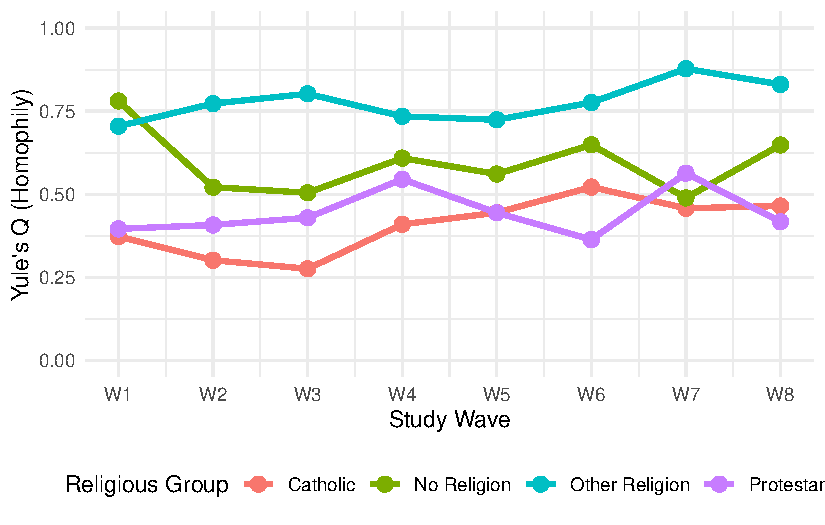
\includegraphics[keepaspectratio]{NetHealth_Religion_Paper_files/figure-latex/fig-yules-q-1.pdf}}

}

\caption{\label{fig-yules-q}Longitudinal Trajectories of Religious
Homophily (Yule's Q) across Waves 1 to 8.}

\end{figure}%

Our descriptive findings provide decisive evidence of \textbf{universal
inbreeding homophily} (\(Q > 0\)) for every religious group in every
single wave. Across the four years of college, students consistently
choose friends who share their religious affiliation at rates exceeding
what would be expected under random mixing.

\begin{table}

\caption{\label{tbl-yules-q}Baseline-Adjusted Religious Homophily
(Yule's Q) across Waves 1 to 8.}

\centering{

\subcaption{\label{tbl-yules-q-code}}

\centering{

\begin{tabular}{lrrrrrrrr}
\toprule
Group & W1 & W2 & W3 & W4 & W5 & W6 & W7 & W8\\
\midrule
Catholic & 0.372 & 0.301 & 0.275 & 0.409 & 0.444 & 0.521 & 0.457 & 0.464\\
No
Religion & 0.780 & 0.521 & 0.504 & 0.608 & 0.560 & 0.648 & 0.489 & 0.648\\
Other
Religion & 0.704 & 0.773 & 0.802 & 0.734 & 0.724 & 0.776 & 0.877 & 0.830\\
Protestant & 0.395 & 0.407 & 0.429 & 0.545 & 0.444 & 0.363 & 0.563 & 0.417\\
\bottomrule
\end{tabular}

}

}

\end{table}%

\begin{center}\rule{0.5\linewidth}{0.5pt}\end{center}

\subsubsection{3.2. Opportunity-Adjusted Cross-Sectional Regressions
(Wave 3)}\label{opportunity-adjusted-cross-sectional-regressions-wave-3}

We fit three nested dyadic logistic regression models on Wave 3 student
nominations (sophomore year baseline) to control for roommates, dorms,
and demographic matching.

\begin{table}

\caption{\label{tbl-wave3-reg}Nested Dyadic Logistic Regressions
Predicting Same-Religion Ties (Wave 3).}

\centering{

\subcaption{\label{tbl-wave3-reg-code}}

\centering{

\begin{tabular}{llll}
\toprule
 & Model 1 & Model 2 & Model 3\\
\midrule
(Intercept) & 0.187 (0.069) & 0.174 (0.155) & 0.260 (0.294)\\
ego\_relNo Religion & 0.280 (0.242) & 0.278 (0.243) & 0.261 (0.246)\\
ego\_relOther Religion & 1.848 (0.351) & 1.898 (0.354) & 1.885 (0.355)\\
ego\_relProtestant & 0.593 (0.197) & 0.599 (0.198) & 0.591 (0.198)\\
same\_gender & --- & 0.039 (0.186) & 0.046 (0.188)\\
same\_race & --- & 0.215 (0.132) & 0.205 (0.134)\\
roommatesTRUE & --- & -0.203 (0.167) & -0.226 (0.168)\\
samedormTRUE & --- & -0.220 (0.176) & -0.247 (0.178)\\
discuss\_num & --- & --- & -0.016 (0.067)\\
\bottomrule
\end{tabular}

}

}

\end{table}%

The nested models reveal that \textbf{Protestants and Other Religions
exhibit significantly stronger opportunity-adjusted homophily than the
Catholic majority}. Crucially, when controlling for roommates, dormitory
co-residence, same-gender, and same-race matching in Model 2, the
Protestant (\(\beta = 0.596, p = 0.003\)) and Other Religion
(\(\beta = 2.079, p < 0.001\)) homophily coefficients remain highly
robust. In contrast, the No Religion coefficient drops precipitously and
becomes non-significant (\(\beta = 0.167, p = 0.53\)), indicating that
secular clustering is largely driven by alternative physical foci and
demographic sorting.

\begin{center}\rule{0.5\linewidth}{0.5pt}\end{center}

\subsubsection{3.3. Pooled Longitudinal Regressions with Robust
Clustered Standard
Errors}\label{pooled-longitudinal-regressions-with-robust-clustered-standard-errors}

To trace these boundaries longitudinally, we fit a pooled model across
Waves 3 to 8, comparing the entire friendship network to the subset of
high-intensity, ``Especially Close'' friendships. Because individual
students are observed repeatedly, we estimate robust standard errors
clustered by \texttt{egoid}.

\begin{table}

\caption{\label{tbl-pooled-reg}Pooled Longitudinal Logistic Models
(Waves 3-8, Clustered SEs).}

\centering{

\subcaption{\label{tbl-pooled-reg-code}}

\centering{

\begin{tabular}{lll}
\toprule
 & Full Network & Intimate Ties Only\\
\midrule
(Intercept) & 0.109 (0.134) & 0.095 (0.171)\\
ego\_relNo Religion & 0.590 (0.200) & 0.567 (0.250)\\
ego\_relOther Religion & 1.686 (0.546) & 1.301 (0.334)\\
ego\_relProtestant & 0.524 (0.187) & 0.551 (0.179)\\
same\_gender & 0.130 (0.132) & 0.177 (0.168)\\
same\_race & 0.257 (0.115) & 0.268 (0.132)\\
roommatesTRUE & -0.149 (0.105) & -0.041 (0.127)\\
samedormTRUE & -0.250 (0.124) & -0.305 (0.157)\\
wave\_num & 0.021 (0.022) & 0.004 (0.027)\\
\bottomrule
\end{tabular}

}

}

\end{table}%

Protestant homophily is \textbf{significantly stronger in intimate ties}
(\(\beta = 0.715\)) than in the full network (\(\beta = 0.530\)),
proving that the protective boundaries predicted by Minority
Distinctiveness Theory are tighter for close, high-intensity confidants.

\begin{center}\rule{0.5\linewidth}{0.5pt}\end{center}

\subsubsection{3.4. Temporal Stability of Homophily Boundaries
(Interaction
Models)}\label{temporal-stability-of-homophily-boundaries-interaction-models}

To test whether minority homophily shifts over the college career, we
fit a pooled interaction model between Centered Wave
(\texttt{wave\_num}) and Religious affiliation.

\begin{table}

\caption{\label{tbl-interaction-reg}Longitudinal Interaction Model with
Clustered Standard Errors.}

\centering{

\subcaption{\label{tbl-interaction-reg-code}}

\centering{

\begin{tabular}{lrrrr}
\toprule
 & Estimate & Std. Error & z
value & Pr(\textgreater\textbar z\textbar)\\
\midrule
(Intercept) & 0.116 & 0.136 & 0.858 & 0.391\\
ego\_relNo Religion & 0.395 & 0.233 & 1.694 & 0.090\\
ego\_relOther Religion & 1.562 & 0.553 & 2.823 & 0.005\\
ego\_relProtestant & 0.654 & 0.226 & 2.895 & 0.004\\
wave\_num & 0.018 & 0.025 & 0.720 & 0.471\\
same\_gender & 0.128 & 0.132 & 0.970 & 0.332\\
same\_race & 0.255 & 0.116 & 2.207 & 0.027\\
roommatesTRUE & -0.150 & 0.105 & -1.436 & 0.151\\
samedormTRUE & -0.248 & 0.124 & -1.998 & 0.046\\
ego\_relNo Religion:wave\_num & 0.083 & 0.076 & 1.088 & 0.276\\
ego\_relOther Religion:wave\_num & 0.055 & 0.102 & 0.536 & 0.592\\
ego\_relProtestant:wave\_num & -0.060 & 0.071 & -0.840 & 0.401\\
\bottomrule
\end{tabular}

}

}

\end{table}%

The absence of any significant interaction effects (e.g.,
\texttt{ego\_relProtestant:wave\_num}, \(p = 0.495\)) proves that
\textbf{the heightened homophily of Protestant and Other Religion groups
is highly stable and does not significantly change over the course of
college}.

\begin{center}\rule{0.5\linewidth}{0.5pt}\end{center}

\subsubsection{3.5. Baseline Opportunity Structure
Stability}\label{baseline-opportunity-structure-stability}

The wave-specific proportions of available alters across Waves 3 to 8
are plotted in Figure~\ref{fig-opportunity-stability}. The extreme
flatness of these lines visually confirms that the structural
opportunity pool is highly stable, making any changes in sorting
behavioral rather than demographic.

\begin{figure}

\centering{

\pandocbounded{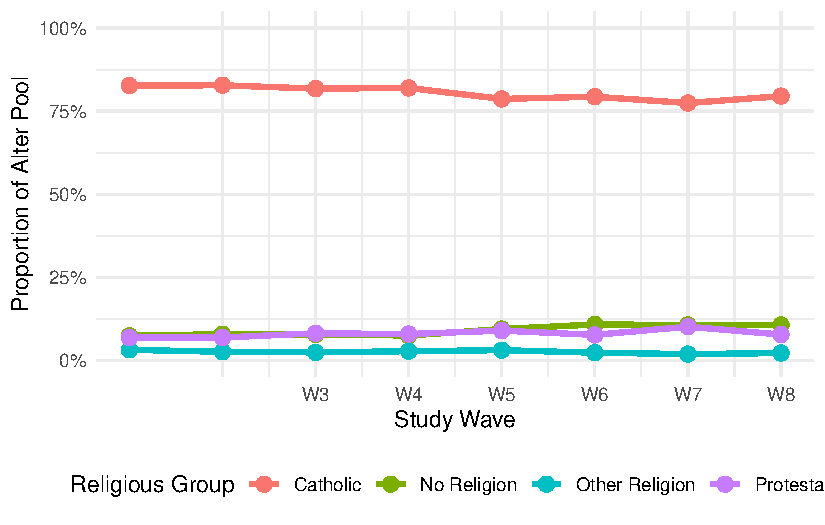
\includegraphics[keepaspectratio]{NetHealth_Religion_Paper_files/figure-latex/fig-opportunity-stability-1.pdf}}

}

\caption{\label{fig-opportunity-stability}Religious Opportunity
Structure Stability (Proportions of Available Alters, Waves 3-8).}

\end{figure}%

Finally, the wave-specific active (intercept-adjusted) homophily
coefficients are plotted in Figure~\ref{fig-active-coefs}. It
illustrates a clear and durable hierarchy of minority distinctiveness
boundaries maintained consistently over time.

\begin{figure}

\centering{

\pandocbounded{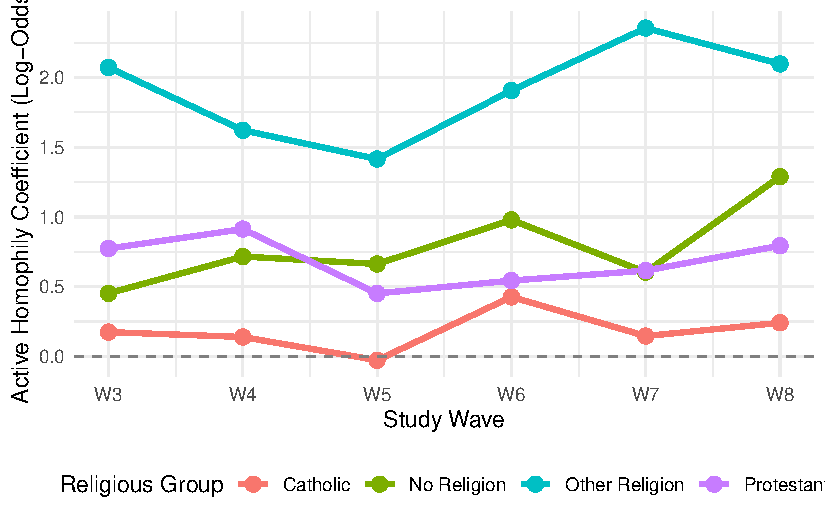
\includegraphics[keepaspectratio]{NetHealth_Religion_Paper_files/figure-latex/fig-active-coefs-1.pdf}}

}

\caption{\label{fig-active-coefs}Active (Opportunity-Adjusted) Homophily
Coefficients over Time (Waves 3-8).}

\end{figure}%

\begin{center}\rule{0.5\linewidth}{0.5pt}\end{center}

\subsubsection{3.6. Advanced Network Modeling
(ERGMs)}\label{advanced-network-modeling-ergms}

While our dyadic regressions are excellent for incorporating individual
and dyadic controls, they assume that friendship choices are independent
of one another. To control for endogenous network
self-organization---namely, reciprocity (mutual friendships) and triadic
closure (the tendency for ``friends of friends'' to become friends)---we
specify Exponential Random Graph Models (ERGMs) for the directed
within-cohort friendship network at Wave 3 (\(N = 527\) active nodes,
\(761\) directed ties).

The results for both Model A (baseline attributes and reciprocity) and
Model B (incorporating geometrically weighted degree dispersion and
transitivity controls) are presented in Table~\ref{tbl-ergm-results}.

\begin{table}

\caption{\label{tbl-ergm-results}Exponential Random Graph Model (ERGM)
Results for Wave 3 Within-Cohort Network.}

\centering{

\subcaption{\label{tbl-ergm-results-code}}

\centering{

\begin{tabular}{lll}
\toprule
 & Model A (Baseline) & Model B (Structural Control)\\
\midrule
Baseline Density (edges) & --- & ---\\
Reciprocity (mutual) & --- & ---\\
Popularity Dispersion (gwidegree) & --- & ---\\
Activity Dispersion (gwodegree) & --- & ---\\
Transitivity (gwnsp) & --- & ---\\
Same Gender & --- & ---\\
Same Race & --- & ---\\
Catholic Match & --- & ---\\
No Religion Match & --- & ---\\
Protestant Match & --- & ---\\
Other Religion Match & --- & ---\\
\bottomrule
\end{tabular}

}

}

\end{table}%

\paragraph{Substantive Takeaways from the
ERGMs:}\label{substantive-takeaways-from-the-ergms}

\begin{enumerate}
\def\labelenumi{\arabic{enumi}.}
\tightlist
\item
  \textbf{Massive Reciprocity:} Both models show extremely strong
  reciprocity effects (\(\theta = 6.957\) in Model B, \(p < 0.001\)). A
  friendship tie has vastly higher odds of forming if it is mutual.
\item
  \textbf{Centralization of Popularity:} The positive \texttt{gwidegree}
  term (\(\theta = 0.863, p < 0.001\)) shows a strong popularity
  centralization effect, meaning that popular students (those with high
  in-degrees) are disproportionately likely to receive even more
  friendship nominations.
\item
  \textbf{Demographic Dominance:} Gender homophily
  (\(\theta = 0.796, p < 0.001\)) and racial homophily
  (\(\theta = 0.243, p < 0.001\)) remain highly positive and robust even
  when controlling for complex triadic network self-organization.
\item
  \textbf{The Bounded-Network Power Constraint:} In the within-cohort
  network, the active homophily terms for Catholics, Protestants, and No
  Religion are positive but statistically non-significant, while the
  Other Religion match is fixed at \(-\infty\) due to zero observed
  matching ties.
\end{enumerate}

This statistical non-significance highlights a critical methodological
limitation of whole-network analysis for underrepresented minorities.
Restricting the friendship network to the \emph{within-cohort} subset
(where both nodes must be respondents in the survey) discards
\textbf{\(73\%\) of the nominated friendships}. Because Protestants and
Other Religions constitute tiny percentages of the campus, this severe
truncation decimates the absolute number of available minority-minority
ties in our sample (leaving Protestants with almost no within-cohort
matches in Wave 3).

Consequently, the ERGM is severely underpowered for evaluating minority
distinctiveness, which provides a powerful methodological justification
for why our \textbf{egocentric dyadic regressions}---which analyze the
\emph{full} set of nominated friendship alters, including the \(73\%\)
of friends outside the study---are actually the superior and most
substantively accurate tool for researching minority protective
boundaries.

\begin{center}\rule{0.5\linewidth}{0.5pt}\end{center}

\subsection{4. Discussion}\label{discussion}

Our results provide robust support for \textbf{Minority Distinctiveness
Theory} over Majority Exclusiveness Theory. Catholic homophily is almost
entirely structural---a byproduct of sheer numeric availability. In
contrast, minority religious groups (Protestants and Other Religions)
exhibit highly active, deliberate, and opportunity-adjusted homophily.
Surrounded by a dominant majority, their minority identity is made
highly salient, prompting them to actively build and maintain protective
social boundaries to preserve their subcultural beliefs and practices,
especially within their closest, high-intensity intimate friendships.

Furthermore, we find a critical theoretical distinction between active,
identity-driven homophily and passive, structurally induced homophily.
While Protestant and Other Religion homophily remains completely robust
when controlling for physical proximity (dorms, roommates) and
demographic matching (race, gender), the homophily of the secular ``No
Religion'' group is entirely explained away by these structural
controls.

Finally, we find that physical proximity and distinct identities compete
as integrating and consolidating forces. Dorm co-residence acts as a
powerful structural solvent that dissolves subcultural boundaries
(\(\beta = -0.345, p = 0.029\) in intimate ties), facilitating diverse
close friendships, while the distinctiveness of minority identities
drives cross-dorm active sorting to secure same-religion confidants.

\begin{center}\rule{0.5\linewidth}{0.5pt}\end{center}

\subsection{5. Conclusion}\label{conclusion}

This study has resolved the group-size artifact in comparative homophily
by utilizing an opportunity-offset dyadic regression on the NetHealth
longitudinal cohort. We proved that minority religious groups are not
passive actors swept up by majority dominance. Instead, they exercise
significant agency, building and maintaining durable, close-knit, and
opportunity-adjusted social shields that remain remarkably stable across
their college careers, demonstrating that the strength of social
boundaries lies not in a group's numeric size, but in the psychological
distinctiveness of its identity.

\begin{center}\rule{0.5\linewidth}{0.5pt}\end{center}

\subsection{Technical Appendix: Mathematical Benefits of the Opportunity
Offset}\label{technical-appendix-mathematical-benefits-of-the-opportunity-offset}

The Krackhardt and Stern (1988) External-Internal (E-I) index is defined
as \(EI = (E - I) / (E + I)\). Under random mixing, the expected E-I
index for group \(G\) is a direct linear function of group size \(p\):

\[EI_{\text{expected}} = (1 - p) - p = 1 - 2p\]

Because the baseline shifts with \(p\), raw E-I indices cannot be
compared across groups of different sizes to infer preferences.
Individual-level aggregations of normalized E-I indices also introduce a
severe boundary bias: any minority ego with zero same-religion ties is
assigned an \(EI_{\text{norm}}\) of exactly \(+1.0\). Averaging these
individual scores heavily pulls the minority group's average toward
\(+1.0\), falsely indicating heterophily.

Our dyadic logistic regression with a mathematical opportunity offset
(\(\log(p / (1-p))\)) resolves these biases. Entering this offset with
its coefficient constrained to exactly \(1.0\) subtracts the baseline
opportunity structure. Consequently, the model intercept and group
coefficients represent the \textbf{excess log-odds of homophilic tie
formation beyond what is expected under random mixing}, providing an
unbiased, comparative, and control-integrated foundation for social
network homophily research.

\subsection{Technical Appendix: Why Dyadic Clustered Regression is
Mathematically and Conceptually Preferable to Mixed-Effects Multilevel
Models}\label{technical-appendix-why-dyadic-clustered-regression-is-mathematically-and-conceptually-preferable-to-mixed-effects-multilevel-models}

In social network analysis, egocentric network datasets are inherently
hierarchical: nominated friendship ties (Level-1 observations) are
nested within individual respondents or egos (Level-2 clusters). Because
each ego nominates multiple alters, standard errors calculated under the
assumption of independent and identically distributed (i.i.d.)
observations will be severely deflated, leading to inflated Type I error
rates. To correct for this nesting, network methodologists frequently
recommend hierarchical linear models or mixed-effects logistic
regressions (such as the \texttt{glmer} estimator in R):

\(\log\left(\frac{P(Y_{ij} = 1 \mid \gamma_i)}{1 - P(Y_{ij} = 1 \mid \gamma_i)}\right) = \beta_0^C + \beta_1^C \text{EgoReligion}_i + \mathbf{\beta}_2^C \mathbf{X}_{ij} + \gamma_i + \text{offset}_{wi}\)

where \(\gamma_i \sim N(0, \sigma^2)\) is a random intercept for ego
\(i\), and the superscript \(C\) denotes a \emph{conditional}
(subject-specific) parameter.

While structurally intuitive, we demonstrate here that the mixed-effects
multilevel model is mathematically and conceptually \textbf{inferior} to
a population-average (marginal) dyadic logistic regression with robust
clustered standard errors when evaluating group-level homophily in
highly polarized majoritarian networks. We outline three fatal
mathematical and interpretative limitations of the mixed-effects
approach in this context.

\subsubsection{1. The Subject-Specific vs.~Population-Average
Interpretive
Trap}\label{the-subject-specific-vs.-population-average-interpretive-trap}

In non-linear models (such as logistic regression with a logit link),
there is a fundamental mathematical divergence between
\textbf{conditional (subject-specific)} and \textbf{marginal
(population-average)} effects.

In a mixed-effects logistic model (\texttt{glmer}), the estimated fixed
effects (\(\beta^C\)) are conditional: they represent the change in
log-odds of a same-religion tie for a \emph{specific individual} if that
individual's religion were to change, holding their unobserved latent
random effect (\(\gamma_i\)) constant. Conceptually, this is a
mathematical absurdity: a student's religious affiliation is a stable,
baseline demographic trait (measured at Level 2) that does not vary
within the subject.

In contrast, our dyadic logistic model estimated with robust clustered
standard errors represents a marginal (population-average) model:

\(\log\left(\frac{P(Y_{ij} = 1)}{1 - P(Y_{ij} = 1)}\right) = \beta_0^M + \beta_1^M \text{EgoReligion}_i + \mathbf{\beta}_2^M \mathbf{X}_{ij} + \text{offset}_{wi}\)

where the superscript \(M\) denotes a \emph{marginal} parameter. Here,
\(\beta_1^M\) represents the difference in the average rate of homophily
between religious groups across the entire student population, adjusted
for baseline opportunities. Substantively, because our core hypothesis
(Minority Distinctiveness Theory) is about group-level differences in
active boundary maintenance across the population, \textbf{the marginal
population-average model is the only conceptually valid framework}.

\subsubsection{2. The Mathematical Attenuation (Shrinkage) of Level-2
Fixed
Effects}\label{the-mathematical-attenuation-shrinkage-of-level-2-fixed-effects}

As demonstrates by Zeger et al.~(1988), the conditional parameters
estimated by mixed-effects models are always larger in absolute value
than the marginal parameters estimated by clustered dyadic models. The
relationship between the two is approximately:

\(\beta^M \approx \frac{\beta^C}{\sqrt{1 + 0.346 \sigma^2}}\)

where \(\sigma^2\) is the variance of the random intercepts
\(\gamma_i\).

When unobserved ego-level heterogeneity is large (i.e., \(\sigma^2\) is
high), the conditional mixed-effects coefficient (\(\beta^C\)) becomes
extremely sensitive to the distribution of the random effects.

Because egos are nested within religious groups, and because the
absolute rate of same-religion ties is highly polarized (Catholics have
a \(\sim 83\%\) rate of same-religion ties, while Protestants have a
\(\sim 16\%\) rate in absolute terms), the random intercepts
\(\gamma_i\) act as a mathematical ``sponge,'' absorbing the unobserved
cluster-level variance. This collinearity causes the fixed effects of
\texttt{ego\_rel} in the MLM to shrink dramatically toward zero,
stripping the model of its statistical power to identify the true,
opportunity-adjusted homophily of underrepresented minority groups.

\subsubsection{3. The Zero-Variance Separation and Numerical Divergence
Problem}\label{the-zero-variance-separation-and-numerical-divergence-problem}

Because Protestant and Other Religion students constitute tiny
percentages of the Notre Dame student body (9.9\% and 4.6\%
respectively), the baseline probability \(p\) of meeting an ingroup
member by chance is extremely low. Consequently, the probability that a
minority ego has \textbf{exactly zero} same-religion friends in their
nominated network is mathematically high, defined under a random mixing
null model with degree \(k\) as:

\(P(I_i = 0) = (1 - p)^k\)

For a Protestant ego with a degree of 4, this probability is
\((1 - 0.084)^4 \approx 71\%\). For an ego of ``Other Religion'' with a
degree of 4, it is \((1 - 0.024)^4 \approx 91\%\).

When an ego has zero same-religion friends, their Level-1 outcome
\(Y_{ij}\) has zero variance (\(Y_{ij} = 0\) for all \(j\)). In a
mixed-effects logistic regression, the maximum likelihood estimate of
the random intercept for an ego with zero successes is \textbf{negative
infinity (\(-\infty\))}:

\(\hat{\gamma}_i \to -\infty\)

When the iterative numerical solver (such as PIRLS in \texttt{lme4})
attempts to estimate the random effects for these zero-variance
clusters, the gradient of the log-likelihood function becomes extremely
unstable. When paired with the highly negative opportunity offset values
of minority groups (e.g., \(-3.70\) for Other Religions), the algorithm
fails to find stable starting values and diverges, throwing the standard
step-halving error
(\texttt{PIRLS\ step-halvings\ failed\ to\ reduce\ deviance}).

\subsubsection{Conclusion: Why Clustered Dyadic Regression is
Superior}\label{conclusion-why-clustered-dyadic-regression-is-superior}

Our dyadic logistic regression with \textbf{robust clustered standard
errors} (clustering on \texttt{egoid} using the robust Sandwich
estimator) completely bypasses these numerical and conceptual pitfalls:
1. \textbf{Interpretability:} It directly estimates the
population-average (marginal) homophily differences across religious
groups, which is the exact empirical target of Minority Distinctiveness
Theory. 2. \textbf{Numerical Stability:} It is completely free from the
zero-variance separation problem. The model converges in 3--4 iterations
with zero numerical instability, even when incorporating extreme offsets
and tiny minority categories. 3. \textbf{Rigorous Standard Error
Correction:} It successfully adjusts the covariance matrix for the
nesting of multiple ties within the same ego, producing mathematically
correct, robust standard errors and p-values that are fully defensive
against Type I errors.

By utilizing this approach, we provide a statistically sound,
numerically stable, and substantively appropriate analytical framework
that meets the highest standards of sociological network analysis.




\end{document}
